\documentclass[11pt,]{article}
\usepackage[]{mathpazo}
\usepackage{amssymb,amsmath}
\usepackage{subcaption}
\usepackage{ifxetex,ifluatex}
\usepackage{fixltx2e} % provides \textsubscript
\ifnum 0\ifxetex 1\fi\ifluatex 1\fi=0 % if pdftex
  \usepackage[T1]{fontenc}
  \usepackage[utf8]{inputenc}
\else % if luatex or xelatex
  \ifxetex
    \usepackage{mathspec}
  \else
    \usepackage{fontspec}
  \fi
  \defaultfontfeatures{Ligatures=TeX,Scale=MatchLowercase}
\fi
% use upquote if available, for straight quotes in verbatim environments
\IfFileExists{upquote.sty}{\usepackage{upquote}}{}
% use microtype if available
\IfFileExists{microtype.sty}{%
\usepackage{microtype}
\UseMicrotypeSet[protrusion]{basicmath} % disable protrusion for tt fonts
}{}
\usepackage[margin=1in]{geometry}
\usepackage{hyperref}
\hypersetup{unicode=true,
            pdftitle={Milestone 6},
            pdfborder={0 0 0},
            breaklinks=true}
\urlstyle{same}  % don't use monospace font for urls
\usepackage{natbib}
\bibliographystyle{plainnat}
\usepackage{graphicx,grffile}
\makeatletter
\def\maxwidth{\ifdim\Gin@nat@width>\linewidth\linewidth\else\Gin@nat@width\fi}
\def\maxheight{\ifdim\Gin@nat@height>\textheight\textheight\else\Gin@nat@height\fi}
\makeatother
% Scale images if necessary, so that they will not overflow the page
% margins by default, and it is still possible to overwrite the defaults
% using explicit options in \includegraphics[width, height, ...]{}
\setkeys{Gin}{width=\maxwidth,height=\maxheight,keepaspectratio}
\IfFileExists{parskip.sty}{%
\usepackage{parskip}
}{% else
\setlength{\parindent}{0pt}
\setlength{\parskip}{6pt plus 2pt minus 1pt}
}
\setlength{\emergencystretch}{3em}  % prevent overfull lines
\providecommand{\tightlist}{%
  \setlength{\itemsep}{0pt}\setlength{\parskip}{0pt}}
\setcounter{secnumdepth}{5}
% Redefines (sub)paragraphs to behave more like sections
\ifx\paragraph\undefined\else
\let\oldparagraph\paragraph
\renewcommand{\paragraph}[1]{\oldparagraph{#1}\mbox{}}
\fi
\ifx\subparagraph\undefined\else
\let\oldsubparagraph\subparagraph
\renewcommand{\subparagraph}[1]{\oldsubparagraph{#1}\mbox{}}
\fi

%%% Use protect on footnotes to avoid problems with footnotes in titles
\let\rmarkdownfootnote\footnote%
\def\footnote{\protect\rmarkdownfootnote}

%%% Change title format to be more compact
\usepackage{titling}

% Create subtitle command for use in maketitle
\newcommand{\subtitle}[1]{
  \posttitle{
    \begin{center}\large#1\end{center}
    }
}

\setlength{\droptitle}{-2em}
  \title{Mapping the Risk of International Infectious Disease Spread
    (MRIIDS)}
  \subtitle{A project funded through USAID’s ``Combating Zika and
    Future Threats: A Grand Challenge for Development'' program \\
    Milestone 6: Increased complexity of the simple model to include data from Milestone 5}
  \pretitle{\vspace{\droptitle}\centering\huge}
  \posttitle{\par}
  \author{}
  \preauthor{}\postauthor{}
  \predate{\centering\large\emph}
  \postdate{\par}
  \date{27 November, 2017}

\usepackage{tikz}
\usetikzlibrary{positioning}
\usetikzlibrary{chains}

\begin{document}
\maketitle
\tableofcontents

\newpage
\section{Milestone Description}\label{milestone-description}

Increased complexity of the simple model to include data from Milestone
5. Automated testing and validating procedures implemented where
possible. Explore procedures for multiple models comparison and accounting for
uncertainty.

\section{General Approach}
In Milestone 4, we presented a simple transmission model that made us of
historical case counts (data stream 1), information about the
transmissibility of the pathogen (data stream 2) and geographical
characetrisation (data stream 3) as a sole means to predict future risk. 
We built on the simple model presented in Milestone 4 (ML4) to a more
complex model that integrates the information on multiple data streams to provide:

\begin{itemize}
\item estimate model parameters,
\item predict the regional/international spread of Ebola. 
\end{itemize}

We have also established the procedure for the validation process
using historical data and are exploring various possibilities for multi-model comparison.

\section{Presentation of the model}\label{sec:model}

The number of cases at a location \(j\) at time \(t\) is given by the equation
\[
  I_{j, t} \sim Pois\left( \sum_{i = 1}^{n} {\left( p_{i \rightarrow j}
  R_{t, i} \sum_{s = 1}^{t}{I_{i, t - s} w_{s}}\right)} \right),
\]

where \(R_{t, i}\) is the reproduction number at location \(i\) at time
\(t\) and \(p_{i \rightarrow j}\) is the probability of moving from
location \(i\) to location \(j\). The quantity $R_{t, i}$ is the
reproduction number at time $t$ at location $i$. $R_{t, i}$ is
affected by a number of other factors e.g., the intrinsic
transmissibility of a pathogen, the healthcare capacity at location
$i$ etc. Its dependance on these factors is formalised as
\[ R_{t, i} := f(haq_i, R_0, t),\]
where $haq_i$ is an index/score quantifying the healthcare capacity at
$i$, $f$ denotes a function and other symbols have their usual meaning.

The probability of moving between locations is derived from the relative flow of populations between
locations. This latter quantity is estimated using a population flow
model such as gravity model. Under gravity model, the flow of individuals from area \(i\) to area \(j\),
\(\phi_{i \rightarrow j}\), is proportional to the product of the
populations of the two areas, \(N_i\) and \(N_j\), and inversely proportional to the distance between them \(d_{i, j}\) raised to some
power $\gamma$. The probability of movement from location \(i\) to
location \(j\) is given by
\[  p_{i \rightarrow j} = (1 - p_{stay}^i) r_{i \rightarrow j}^{spread},\]

where \(p_{stay}^i\) is the probability of staying at location \(i\) and
\(r_{i \rightarrow j}^{spread}\) is the relative risk of spread to a
location \(j\) from a focal location \(i\).
\(r_{i \rightarrow j}^{spread}\) is quantified as \[
  r_{i \rightarrow j}^{spread} = \frac{\phi_{i \rightarrow
  j}}{\sum_{x}{\phi_{i \rightarrow
  j}}}.
\]

\subsection{Statistical inference of model parameters}
The parameters of the full model as presented in Section~\ref{sec:model} are: $R_{t, i}$, $p_{stay}$ and $\gamma$. The
reproduction number $R_{t, i}$ at time $t$ can be estimated from the
incidence data for the previous 3 to 4 weeks using the package EpiEstim
(\cite{cori2013new}). 

The other parameters can be estimated using maximum likelihood
estimation or estimating the posterior distribution of the parameters using
MCMC. Let the observed incidence time series be $o_1, o_2, \dots
o_t \dots $. Then the likelihood of the model parameters given the
observations is proportional to the probability of the data given
model parameters.  The probability of $o_t$ at time $t$ given
the model parameters is:
\[ P(o_t \mid p_{stay}, \gamma, R_t) = e^-{\lambda_t}
  \frac{o_t^{\lambda_t}}{\lambda_t !}, \]
where $\lambda_t$ is given by
\[\lambda_t = R_t \sum_{s = 1}^t{I_{s}w_{t - s}}.\]

Thus assuming that each observation is independent, the likelihood of the parameters is proportional to
\[
\prod_{t = 1}^{t}{e^-{\lambda_t} \frac{o_t^{\lambda_t}}{\lambda_t !}}.
\]
In practice, we use past 2 to 3 weeks of incidence data to compute the
likelihood.

\subsection{Multi-model Comparison}
We are exploring the use of well established statistical measures ranging from simple such as
likelihood ratio to the more sophisticated information-theoretic
measures such as AIC or DIC for multi-model comparison. Another line
of investigation for multi-model inference is model avaeraging i.e.,
the predicted values are the weighted means of the predictions from
each model under consideration where the weights are the model
probabilities (see \cite{burnham2011aic}). 

\subsection{Predicting Future Incidence Pattern and Geographical Spread}

\section{Implementation Details}

The general approach outlined above relies on several data streams, an
inference framework, and a framework for projection. The code
developed as part of the project will be made available as an open
source R package that will provide functions for pre-processing and
collating the various data streams as well as plug the data into
modules that will do the inference and the projection. 

\begin{figure}
  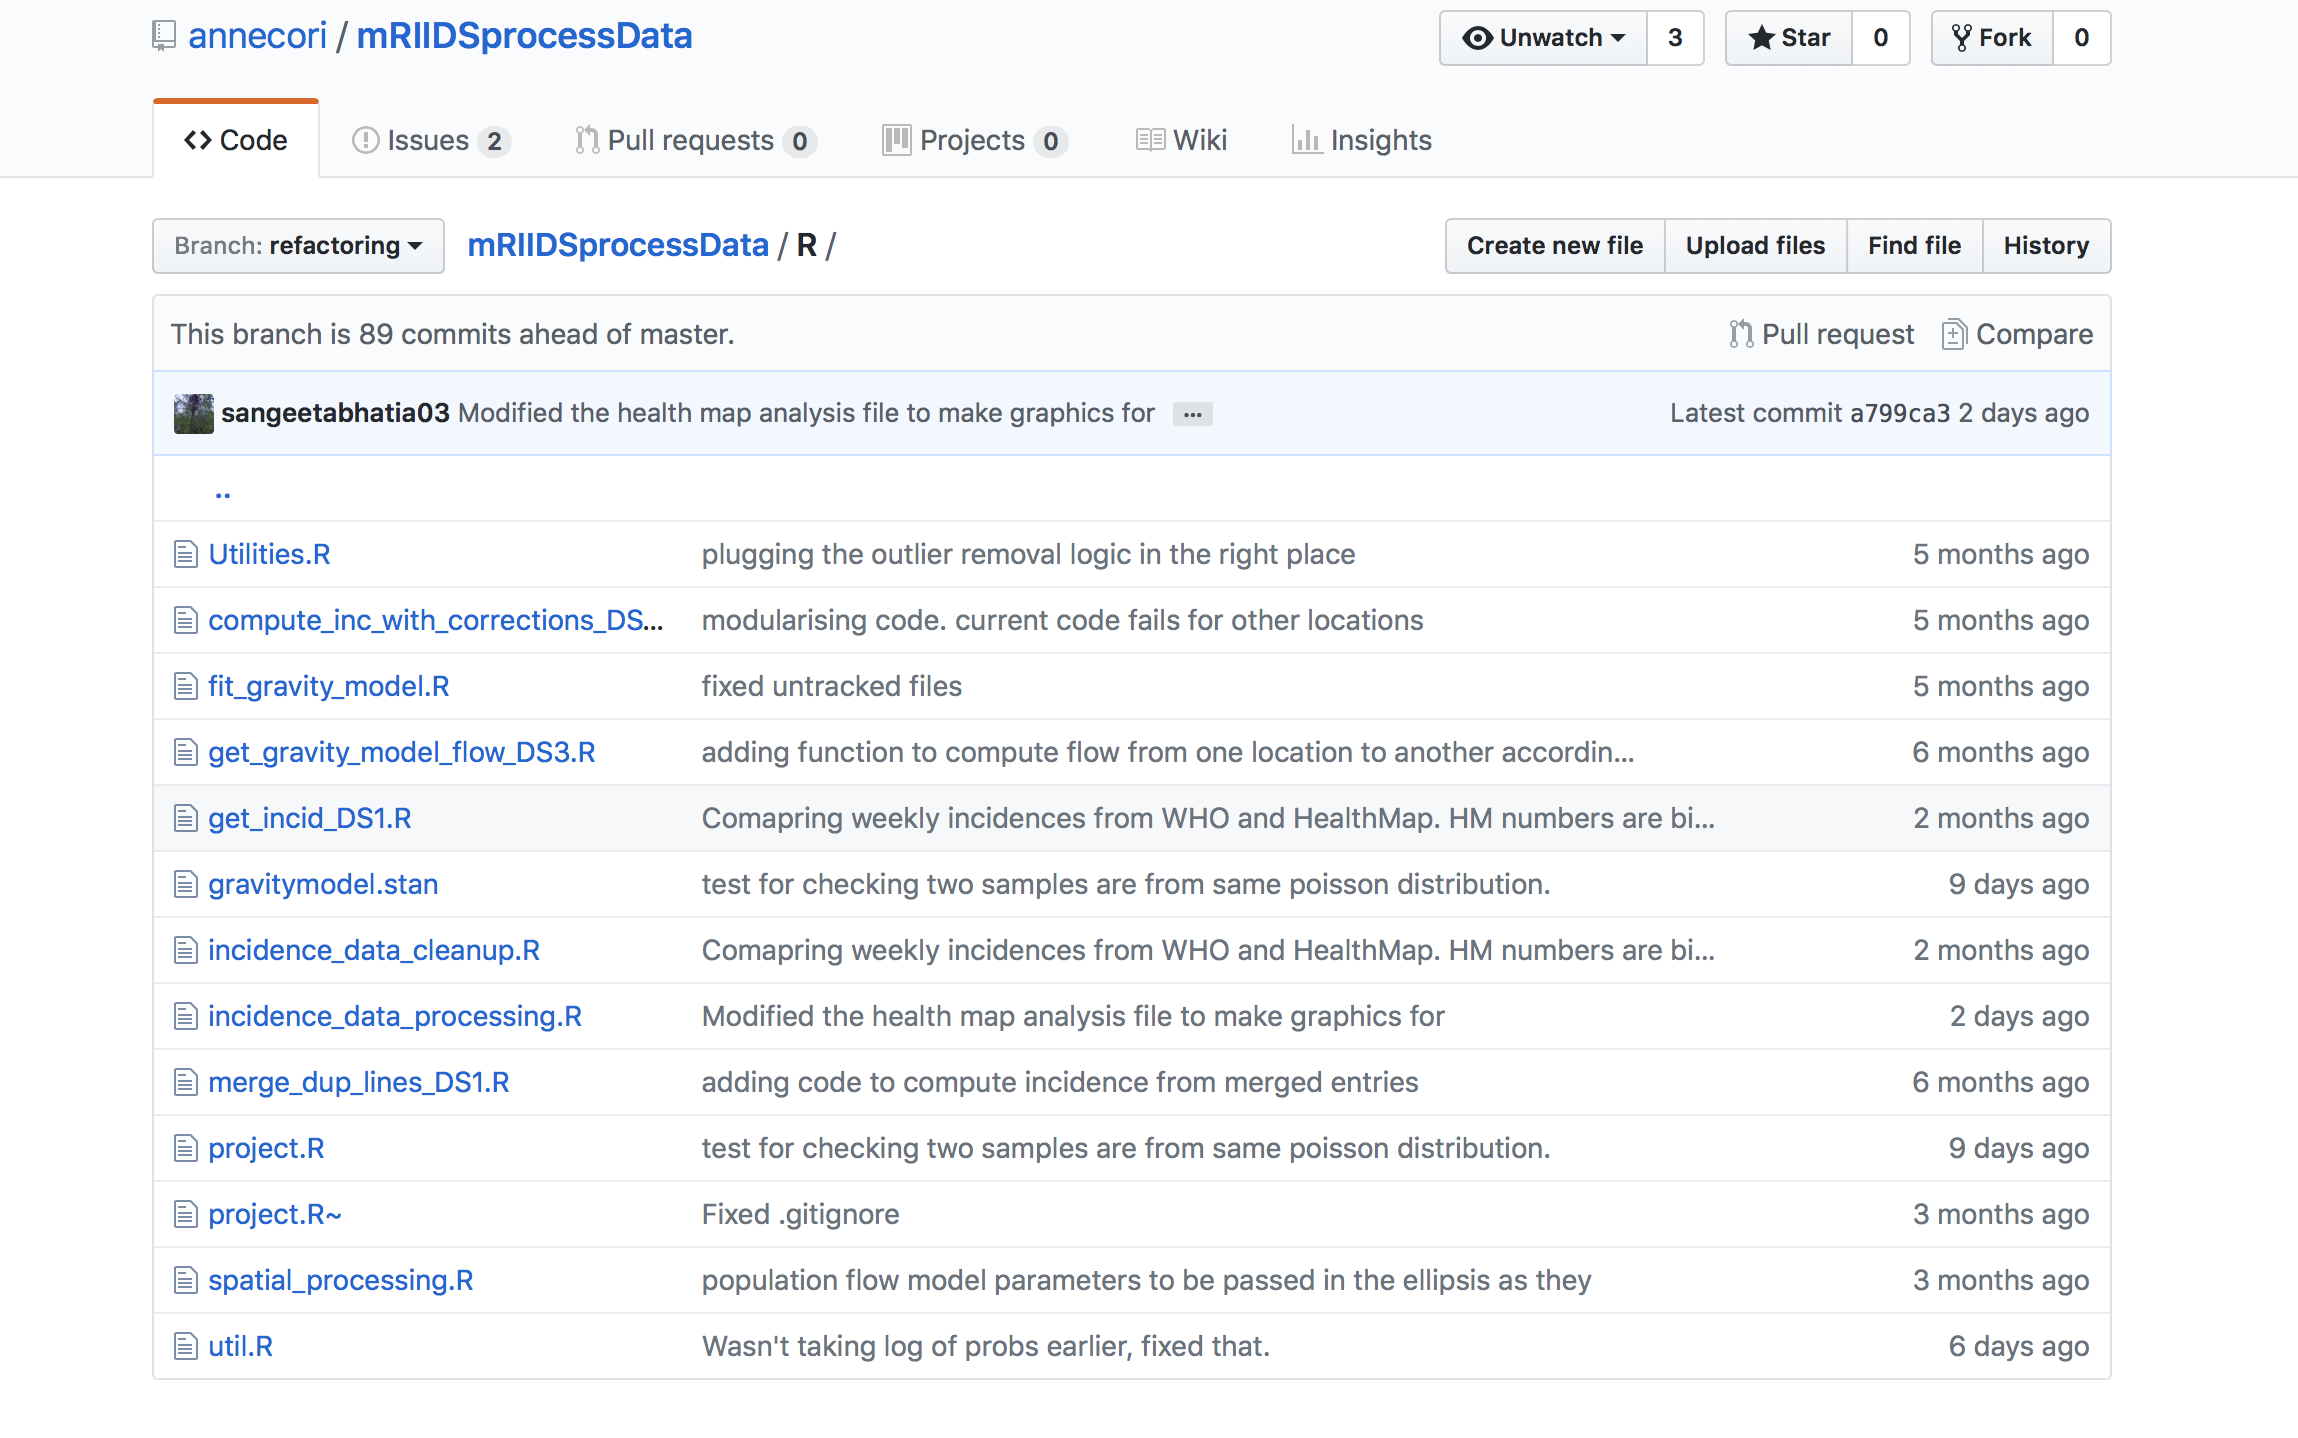
\includegraphics[scale = 0.5]{ms6-figures/github-screenshot}
  \label{fig:github}
  \caption{The software being developed for the project is available
    on GitHub.}
\end{figure}

\subsection{Software Package mRIIDS}
\subsection{Collating data for each data stream}
\begin{center}
\begin{figure}
\begin{tikzpicture}[start chain=1 going right,
                    start chain=2 going left,
                    node distance=5mm,
                    every join/.style=->,
                    every node/.style={draw,
                      rectangle,
                      rounded corners,
                      minimum width = 3.4cm,
                      minimum height = 2cm,
                      text width = 2.3cm,
                      text=black,
                      text opacity=1,
                      align=center,
                    fill=teal!60}]
 \pgfsetfillopacity{0.3}
\node (a) [on chain=1,join] {Extract case counts};
\node (b) [on chain=1,join] {Merge Duplicate Alerts};
\node (c) [on chain=1,join] {Remove outliers};
\node (d) [on chain=1,join] {Discard inconsistent data};
\node (e) [on chain=2, below = of d,join] {Interpolate missing data};
\node (f) [on chain=2,join] {Estimate Reproduction Number};
\node (g) [on chain=2,join] {Determine probability of movement between
  locations};
\node (h) [on chain=2,join] {Predict future incidence};
\draw[->] (d) -- (e);
\end{tikzpicture}
\label{fig:workflow}
\caption{Workflow for the processing of the various data streams.}
\end{figure}
\end{center}

In Milestone 6, a step was added to the data pre-processing workflow
to remove outliers from data. The removal of outliers was done using Chebyshev Inequality
with sample mean (see~\cite{saw1984chebyshev}). Figure~\ref{fig:wf_example} illustrates the results of each step in the pre-processing steps in the workflow. 
\begin{figure}
  \centering
  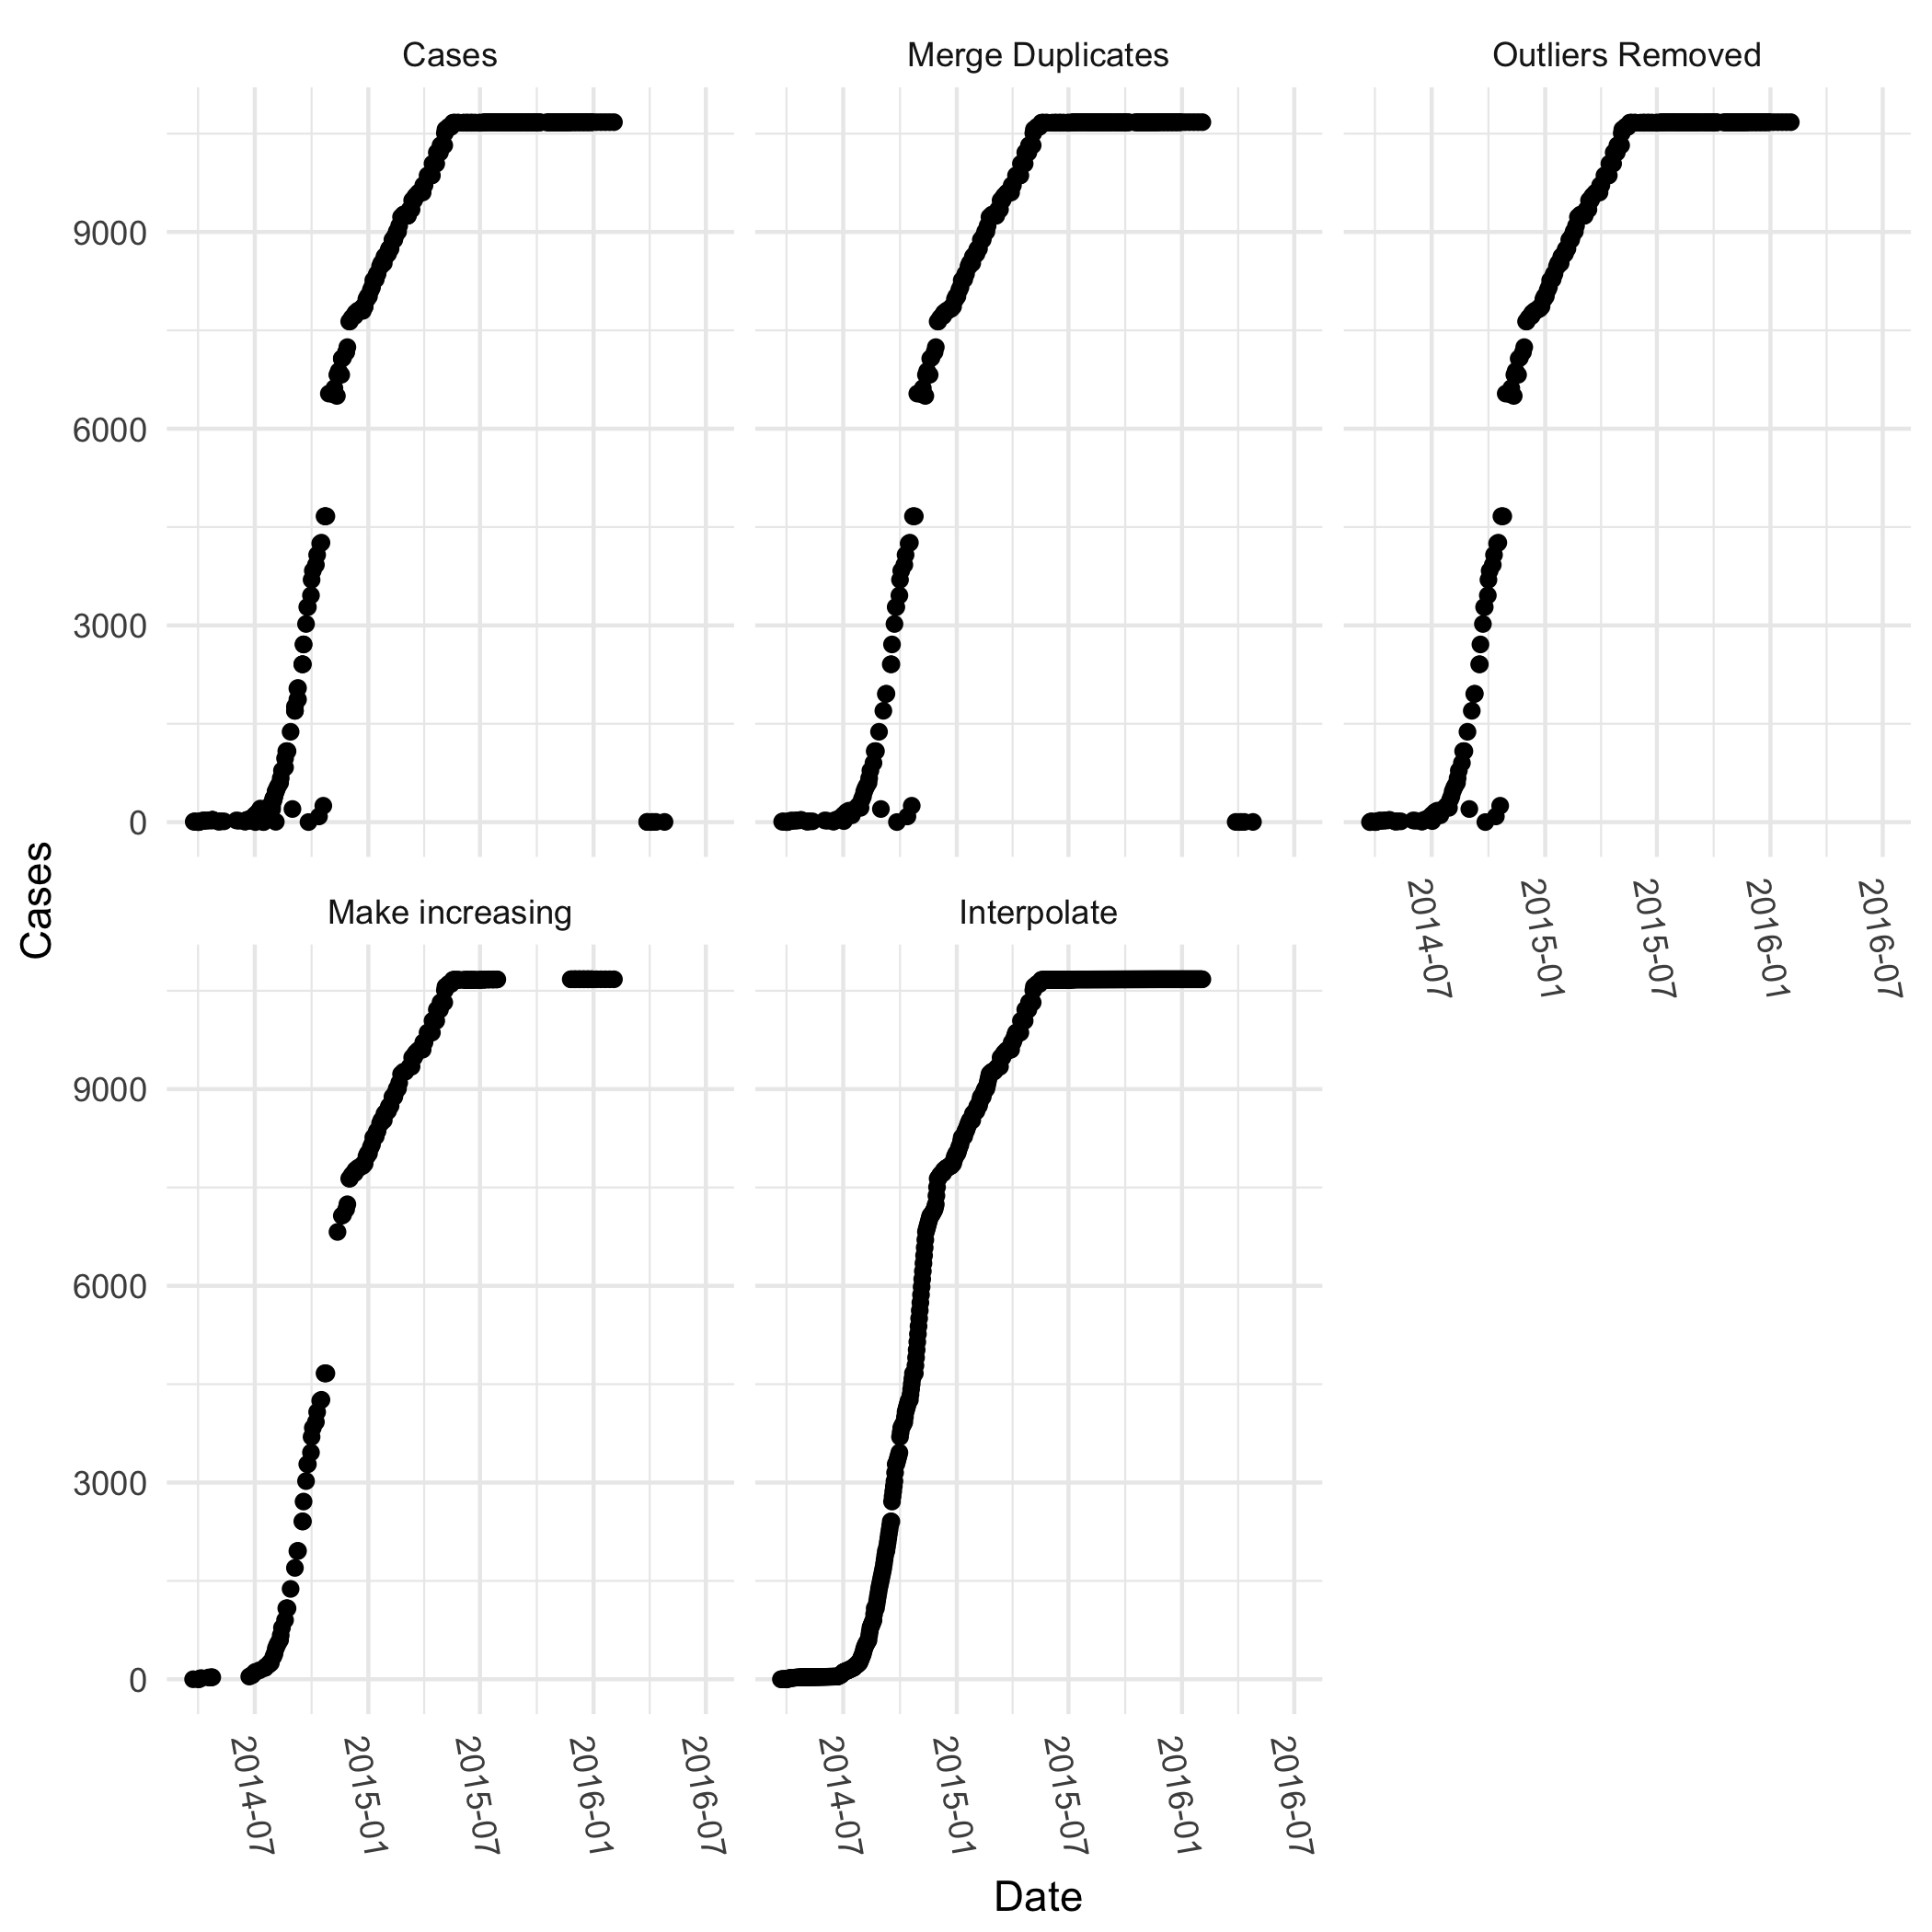
\includegraphics{ms6-figures/liberia-preprocessing.png}
  \caption{Illustration of the pre-processing steps on HealthMap incidence
    data for Liberia.}
  \label{fig:wf_example}
\end{figure}

\subsection{Model training and validation using data from
WHO}\label{model-training-and-validation-using-data-from-who}

In the current iteration, the model was trained and validated the data
on cases officially reported to the WHO during the 2013--2016 Ebola
outbreak in Guinea, Liberia and Sierra Leone. This dataset was cleaned
and published in \citep{garske20160308} and it is this cleaned version
of the data that were used in this work. This dataset consists of
incidence reports at ADM2 level. Thus in using it, we were able to
better validate the model at a finer spatial resolution than available
with HealthMap/ProMed data. We refer to this dataset as WHO data
throughout the rest of this document.

\subsubsection{Incidence trends from different data sources}
We aggregated the WHO data to national level to compare the incidence
trends derived from the three different data sources (WHO, HealthMap
and ProMed). As can be seen in Figures~\ref{fig:incid_comp} and \ref{fig:r_comp}, the
three data sources correlate well both in the incidence time series as
well as the reproduction numbers estimated from the incidence data.
\begin{figure}
    \centering
    \begin{subfigure}[b]{0.8\textwidth}
        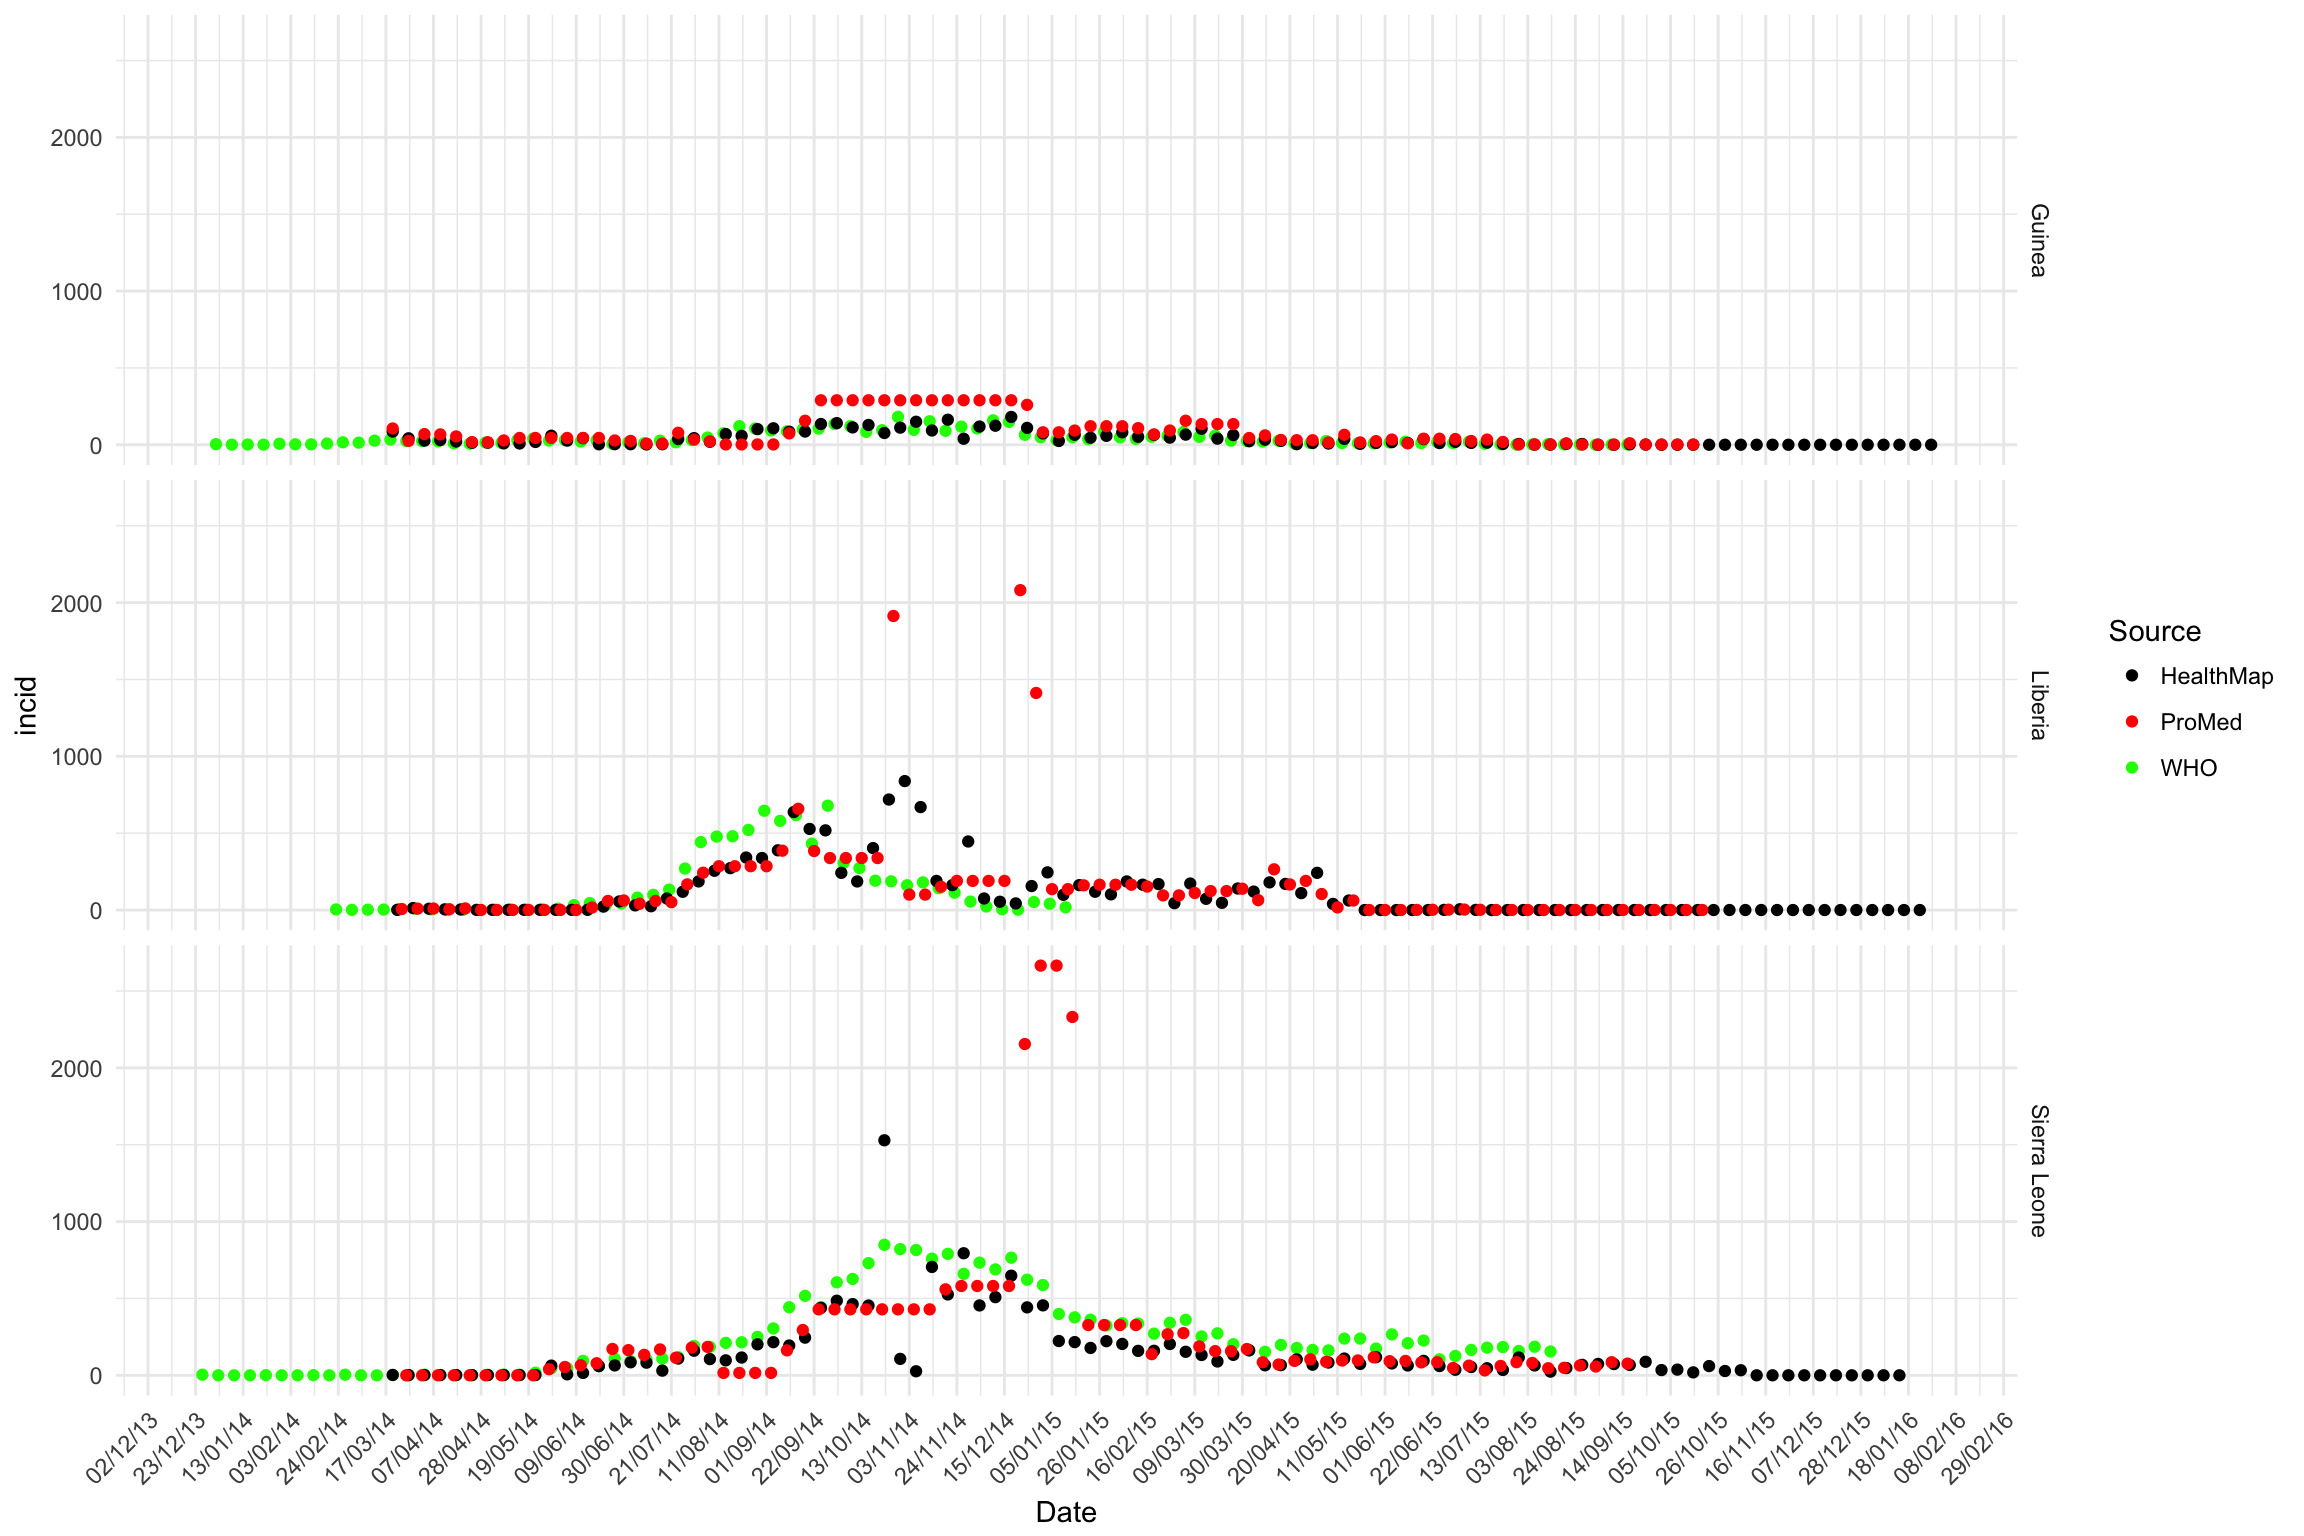
\includegraphics[width=\textwidth]{ms6-figures/who_vs_hm_vs_pm-incid.png}
        \caption{Comparison of incidence data from WHO, HealthMap and ProMed.}
        \label{fig:incid_comp}
      \end{subfigure}
      ~
    \begin{subfigure}[b]{0.8\textwidth}
        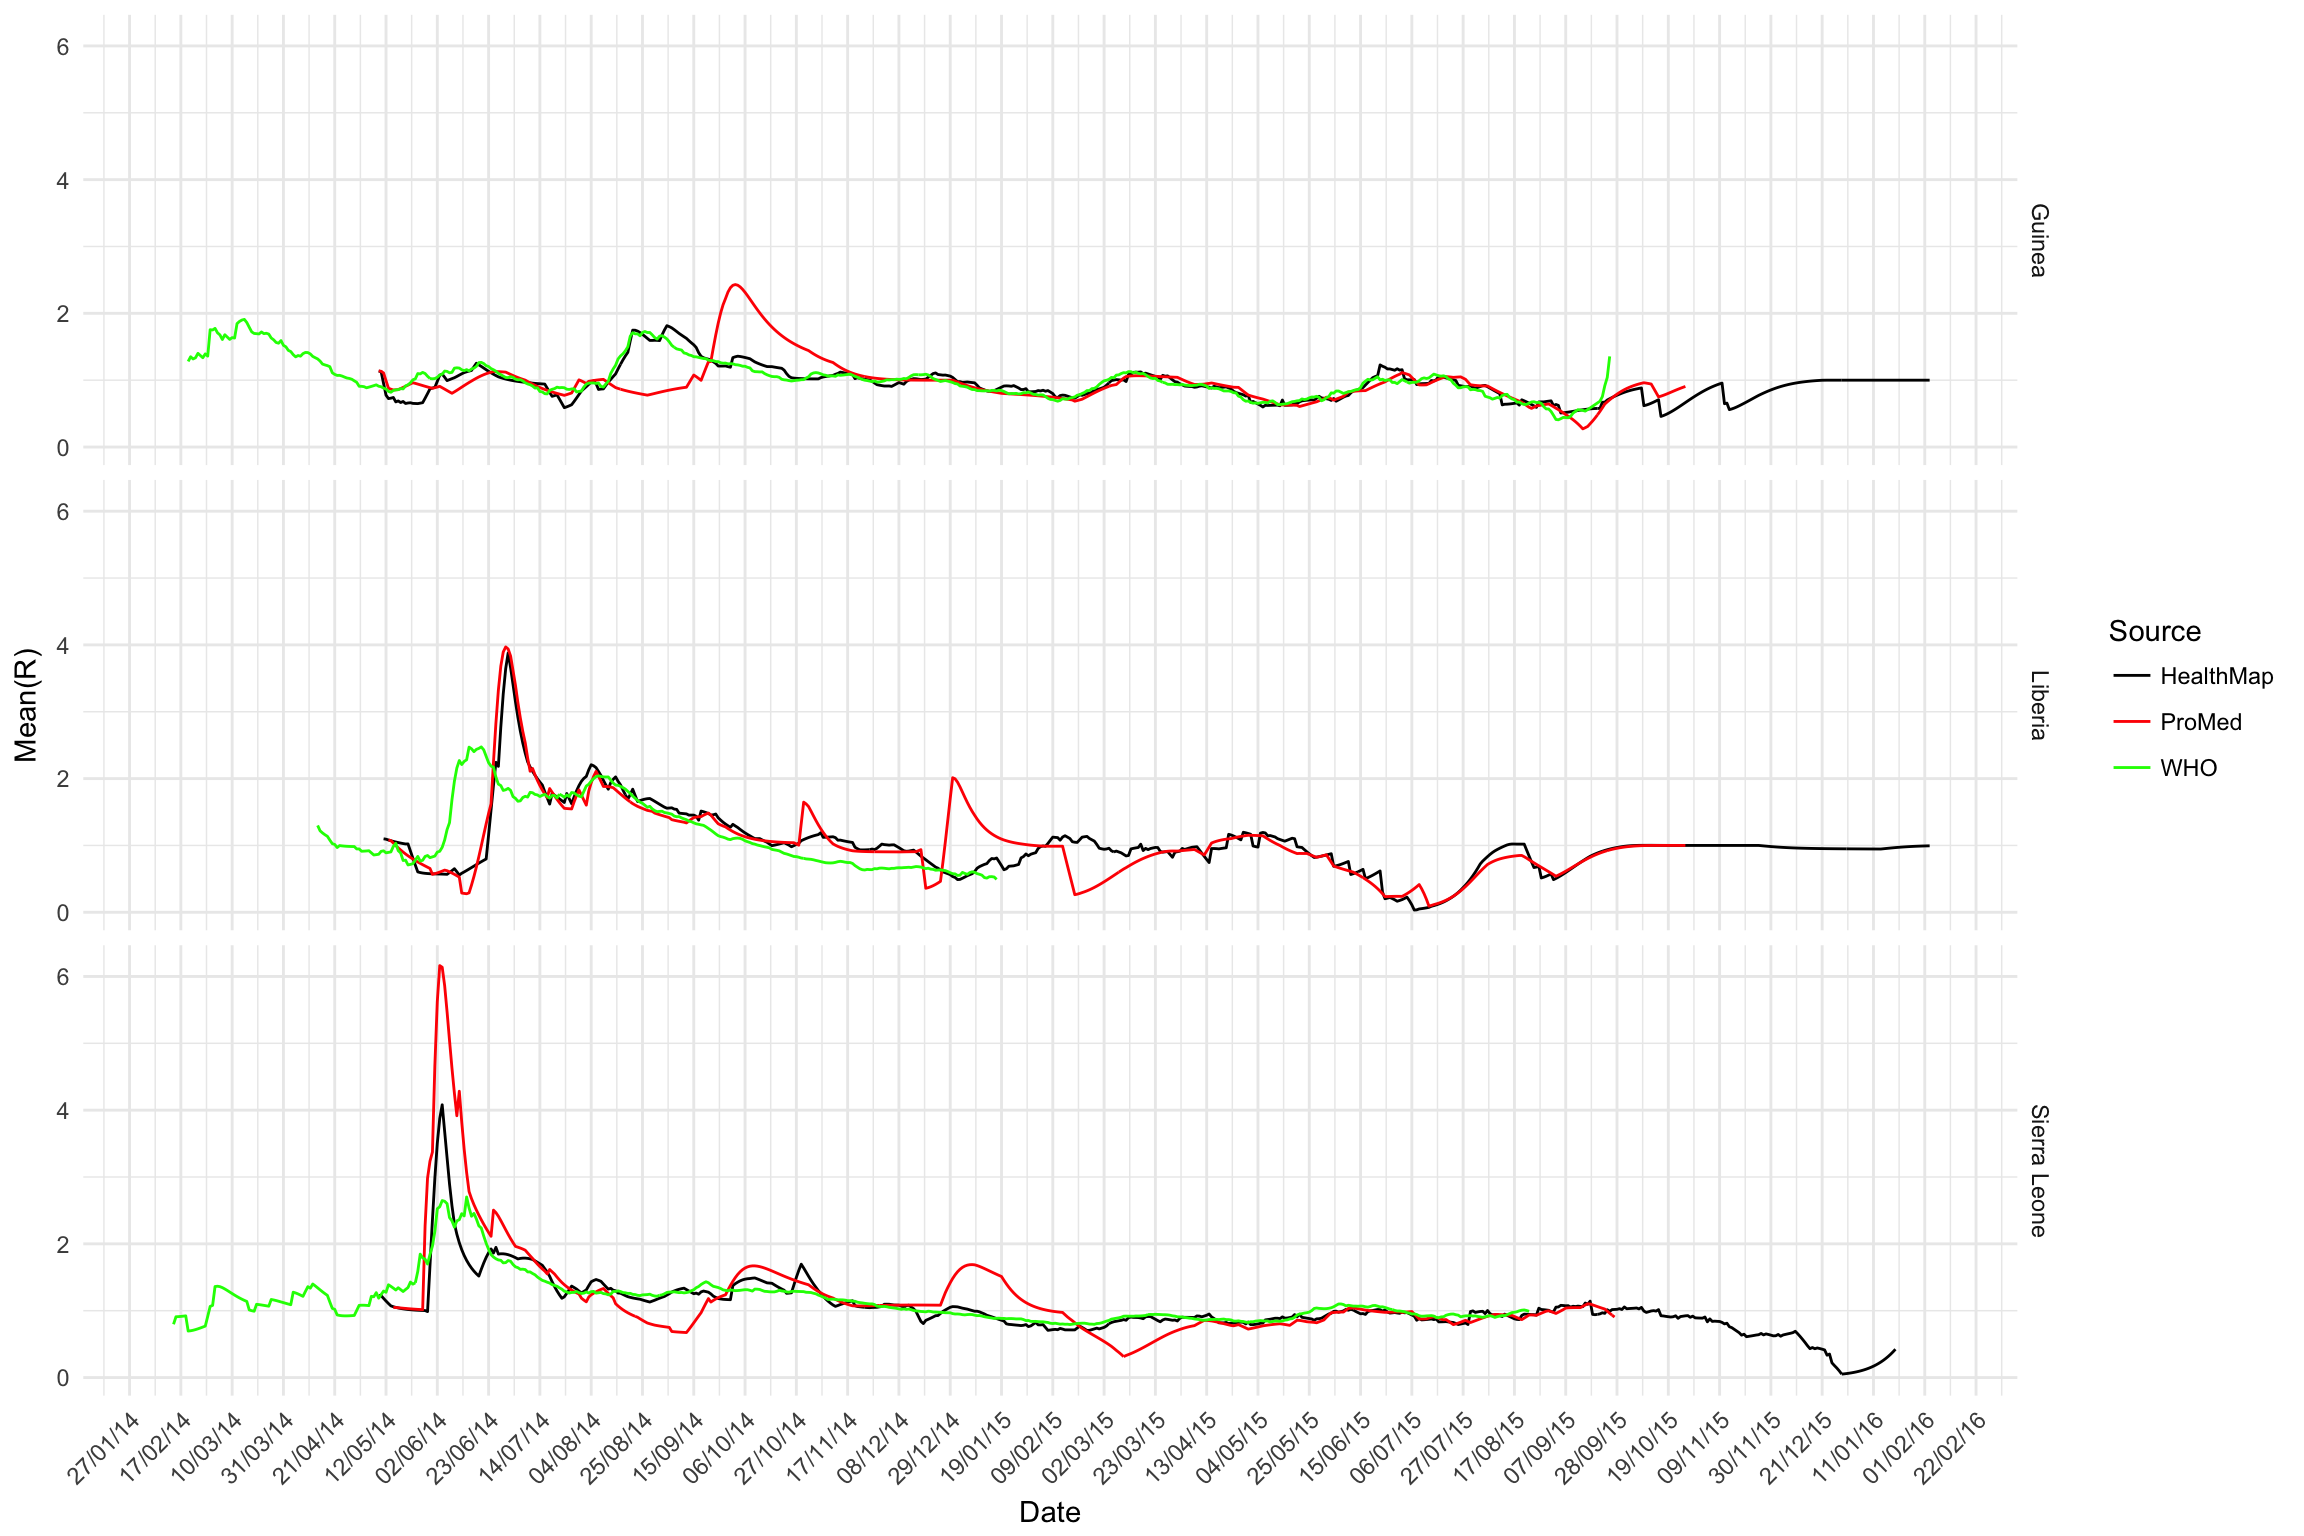
\includegraphics[width=\textwidth]{ms6-figures/who_vs_hm_vs_pm-R.png}
        \caption{Comparison of the reproduction numbers estimated from
        the different sources of the incidence data.}
        \label{fig:r_comp}
    \end{subfigure}
  \end{figure}
  
\section{Output for Ebola in West Africa}\label{output-for-ebola-in-west-africa}



\subsection{Estimating Transmissibility}\label{estimating-transmissibility}

\subsection{Predicting Future Cases}\label{predicting-future-cases}

\subsection{Connectivity and Risk of International
Spread}\label{connectivity-and-risk-of-international-spread}

\subsection{Parameters Inference}
[initial exploration of how $p_{stay}$ and power, using rms]

[Formalization of the likelihood for joint estimation of R, $p_{stay}$, power]

This section should include figures

\subsection{Predicting future incidence and geographical spread}

[present some early results – map of predictions/ incidence curve/ table at country level? ].

\section{Conclusions and next steps}\label{sec:conclusions}







\newpage
\section*{References}
\bibliography{ms6}


\end{document}
